%% LyX 1.6.4 created this file.  For more info, see http://www.lyx.org/.
%% Do not edit unless you really know what you are doing.
\documentclass[12pt,oneside,ngerman]{scrbook}
\usepackage{ae,aecompl}
\usepackage[T1]{fontenc}
\usepackage[utf8]{inputenc}
\setcounter{secnumdepth}{3}
\setcounter{tocdepth}{3}
\usepackage{babel}

\usepackage{array}
\usepackage[unicode=true, pdfusetitle,
 bookmarks=true,bookmarksnumbered=false,bookmarksopen=false,
 breaklinks=false,pdfborder={0 0 1},backref=false,colorlinks=false]
 {hyperref}
\usepackage{graphicx}

\makeatletter

%%%%%%%%%%%%%%%%%%%%%%%%%%%%%% LyX specific LaTeX commands.
%% Because html converters don't know tabularnewline
\providecommand{\tabularnewline}{\\}

\makeatother

\begin{document}

\title{Spezifikation aidGer}


\author{Buchgraber (2512046), Gildein (2513744), Pirrung (2526016)\\
Gruppe 10}

\maketitle
\tableofcontents{}


\chapter{Einleitung\label{cha:Einleitung}}


\section{Zweck\label{sec:Zweck}}

Diese Spezifikation dient als Grundlage für alle weitere Dokumente,
die im Rahmen dieses Softwarepraktikums entstehen. Sie enthält alle
wesentlichen Anforderungen an die Software und deren Schnittstellen.
Sie muss stets mit den anderen Dokumenten, insbesondere dem Entwurf
und der Codierung, konsistent gehalten werden.


\section{Leserkreis\label{sec:Leserkreis}}

Dieses Dokument ist für den folgenden Leserkreis bestimmt:
\begin{itemize}
\item Das gesamte Projektteam
\item Der Kunde
\item Die Betreuer des Softwarepraktikums
\item Der Gutachter des Spezifikationsreview
\item Die künftige Programmierer bzw. Verwalter dieses Projektes
\end{itemize}

\section{Einsatzbereich und Ziele\label{sec:Einsatzbereich-und-Ziele}}

In diesem Projekt soll das Hilfskraftverwaltungssystem ,,aidGer{}``
realisiert werden. Der ,,aidGer{}`` soll den Mitarbeitern der Abteilung
SE die tägliche Arbeit bei der Verwaltung der Hilfskraftbeschäftigungen
des Institutsverbund der Informatik erleichtern.\\
\\
Die neue Software dient grundsätzlich zur Erleichterung der Erfassung
und Auswertung aller Prozesse, die bei der Verwaltung von Hilfskräften
anfallen.\\
\\
Das Ziel ist es, mit ,,aidGer{}`` die jetzige Lösung ,,Hive{}``
zu ersetzen. Sie soll jedoch weiterhin einsetzbar sein, um im Notfall
auf alte Prozesse zurückgreifen zu können.

\section{Fachbegriffe und Abkürzungen}

Alle für dieses Projekt relevanten Fachbegriffe und Abkürzungen sind
im \ref{sec:Begriffslexikon} (im Anhang dieses Dokuments) aufgeführt.

\section{Aufbau dieses Dokuments}

Neben einer allgemeinen Beschreibung des Systems sollen die Anforderungen
an die Funktionen des Systems und die geforderten Qualitäten hinsichtlich
der Software selbst dokumentiert werden. Anschließend wird die Benutzeroberfläche
und die Anwendungsfälle vorgestellt.

\subsection{Konventionen}

In dieser Spezifikation werden die folgenden Konventionen zur Hervorhebung
von Begriffen verwendet:

%TODO: Konventionen festlegen

\chapter{Allgemeine Beschreibung\label{cha:Allgemeine-Beschreibung}}

In diesem Kapitel soll der ,,aidGer{}`` in seinen Grundzügen beschrieben
werden.

\section{Einbettung\label{sec:Einbettung}}

%TODO: Issue #5

Der ``aidGer'' benötigt eine Schnittstelle zur verwendeten 
Datenbank. Diese wird durch die Bibliothek AdoHive zur Verfügung
gestellt. Zudem wird eine Verbindung mit dem bereits vorhandenen
Ticketsystem benötigt.


\section{Grundlegende Funktionen\label{sec:Grundlegende-Funktionen}}

Der ,,aidGer{}`` soll dem Nutzer folgende Grundfunktionen bereitstellen:
\begin{itemize}
\item ..
\end{itemize}
Diese Funktionen sollen für alle Benutzer leicht erlernbar, effizient
und einfach in der Handhabung sein.

\section{Einschränkungen\label{sec:Entwurfseinschr=0000E4nkungen}}

Die Vorgabe des Kunden hinsichtlich der Entwicklungsplattform ist
Java mit der SDK Version 6 als Programmiersprache und Swing als Oberflächenbibliothek.\\

Zur Generierung von PDF-Berichten soll eine aktuelle Version der
iText Bibliothek eingesetzt werden. Um auf die Datenbank zuzugreifen,
soll die von Team AdoHive bereitgestellte AdoHive Bibliothek verwendet
werden. Andere externe Bibliotheken müssen durch den Betreuer explizit
genehmigt werden. Zur Anzeige von den generierten PDF-Berichten muss
der Anwender einen PDF-Betrachter installiert haben. Sollte das Programm
nicht in der Lage sein, den systemspezifischen PDF-Betrachter zu starten,
wird eine entsprechende Meldung dem Benutzer angezeigt.\\

Zur Darstellung von Klassendiagrammen oder ähnlichen Diagrammen,
die während des Entwurfs entstehen, soll UML benutzt werden. \\

Durch den Zeitplan ist ein Prozessmodel bereits vorgegeben.

\pagebreak

\chapter{Anforderungen an die Funktion\label{cha:Anforderungen-an-die}}

In diesem Kapitel werden die funktionalen Anforderungen an das System
im Detail beschrieben.

\section{Leistungsanforderungen\label{sec:Leistungsanforderungen}}

Da das Programm auf dem Computer des Benutzers verwendet wird, sollte
es andere Programme oder das Betriebssystem nicht behindern und alle
Funktionen in möglichst geringer Zeit ($<$ 2 Sekunden) ausführen.

Ausnahmen können hierbei der Export oder das Abspeichern sehr grosser
Sammlungen darstellen.


\section{Mengengerüst\label{sec:Mengenger=0000FCst}}

Folgende Kenngrößen sind für das System relevant:
\begin{itemize}
\item Das Programm ist eine Einzelplatzanwendung ohne Netzwerkfunktionalität
und wird daher stets von einem Anwender bedient.
\end{itemize}

\section{Anforderung: }


\chapter{Benutzeroberfläche\label{cha:Benutzeroberfl=0000E4che}}

Die Benutzeroberfläche des ,,aidGer{}`` soll mit Swing erstellt
werden und sich in das Erscheinungsbild des Betriebssystems einpassen.
Die folgenden Mockups zeigen wie sie ungefähr aussehen soll.

\section{Programmstart}

%TODO: Muss noch mehr hingeschrieben werden

Beim Programmstart wird das Hauptfenster angezeigt. 
Sollten beim vorherigen Schließen des Programms noch Tabs offen gewesen sein, so
wird dem Nutzer die Möglichkeit gegeben diese wieder zu öffnen. Dabei wird versucht
soviele Informationen wie möglichst zu erhalten; Eingaben in Formulare gehen dabei
jedoch verloren.

\section{Titelleiste des Hauptfensters}

In der Titelleiste wird immer der Name der Applikation (``aidGer{}'') sowie die
momentan offene Funktion angezeigt. Dieser Funktionsname stimmt mit dem Titel des
Tabs überein. Ein Beispiel dafür wäre ``Stammdatenverwaltung - aidGer''.

\section{Allgemeine Beschreibung des Hauptfensters}

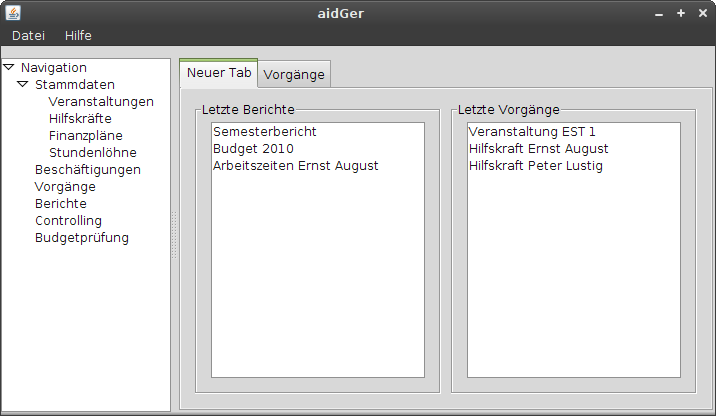
\includegraphics[scale=0.75]{mockup1.png}

Das Hauptfenster ist in zwei Bereiche eingeteilt. Auf der linken Seite befindet
sich die Navigationsleiste in der alle Funktionen angezeigt werden und der Benutzer
einfach zwischen ihnen wechseln kann. Auf der rechten Seite befindet sich der
Inhaltsbereich. Hier wird die aktuell ausgewählte Funktion angezeigt. Im Hintergrund
können zudem noch weitere Funktionen offen sein. Diese befinden sich dann in weiteren
Tabs. Im Beispiel wäre der ``Neue Tab'' der aktuell geöffnete und ``Vorgänge'' ein
sich im Hintergrund befindlicher Tab. \\

Die Navigationsleiste und der Inhaltsbereich sind durch eine bewegliche, vertikale
Leiste getrennt. Dadurch kann die Größe beider Bereiche individuell angepasst werden.

\subsection{Verhalten bei Änderung der Fenstergröße}

Bei einer Veränderung der Fenstergröße in der Breite wird nur der Inhaltsbereich
verändert um mehr Platz für Informationen/Formulare zu bekommen. Die Navigationsleiste
wird höchstens so breit wie das breiteste Element in ihr. \\

Sollte sich die Fenstergröße in der Höhe verändern, ändert sich die Größe beider
Elemente gleichmäßig.

\subsection{Verhalten bei Auswahl eines Elements in der Navigationsleiste}

Wird vom Benutzer ein Element in der Navigationsleiste mit der linken Maustaste 
ausgewählt, wird der aktuelle Inhalt des Inhaltsbereichs verworfen und durch den
Inhalt des neuen Elements ersetzt. \\
Sollte der Benutzer jedoch die mittlere Maustaste benutzen um das Element auszuwählen,
wird ein neuer Reiter geöffnet und der Inhalt des Elements in diesem neuen Reiter
dargestellt. Der aktuelle Reiter bleibt dabei vollständig erhalten, gerät jedoch
in den Hintergrund (ist also nicht mehr sichtbar).

\section{Navigationselemente}

%TODO: Alle Navigationselemente aufzählen

In der folgenden Gliederung der Navigationsleiste sind die obersten Elemente die
Hauptelemente und darunter folgende Sublisten die dementsprechenden Menüs die 
aufklappen sobald man auf das Hauptelement klickt. Nur beim Auswählen der Unterpunkte
wird der Inhalt des Inhaltsbereiches verändert.

\begin{itemize}
    \item Stammdaten
    \begin{itemize}
        \item Veranstaltungen
        \item Hilfskräfte
    \end{itemize}
    
    \item Vorgänge
    \begin{itemize}
        \item Alle anzeigen
        \item Nach Vorgang suchen
    \end{itemize}
\end{itemize}

\section{Menüleiste}

Die Menüleiste befindet sich unter Windows und Linux unterhalb des Fensterrahmens
aber oberhalb der Navigationsleiste und des Inhaltsbereichs. Unter Mac OS X befindet
sie sich in einer Leiste unter dem oberen Bildschirmrand. \\
In der folgenden Gliederung dieser Menüleiste sind die obersten Elemente die
Hauptelemente und darunter folgende Sublisten die dementsprechenden Menüs die 
aufklappen sobald man auf das Hauptelement klickt.

\begin{itemize}
    \item Datei
    \begin{itemize}
        \item Beenden
    \end{itemize}
    \item Hilfe
    \begin{itemize}
        \item Hilfe
        \item Über
    \end{itemize}
\end{itemize}

\section{Programmeinstellungen}

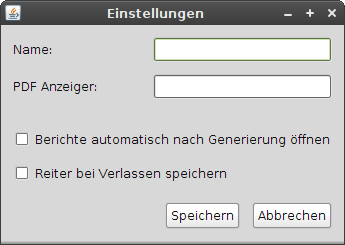
\includegraphics[scale=1.00]{MockupSettings.png}

Das Einstellungsfenster ist ein modaler Dialog, der über keine Menüleiste verfügt.
Ganz unten verfügt er über zwei Buttons. Über den Abbrechen-Button schließt sich
das Fenster ohne die Einstellungen zu speichern. Mit Hilfe des Speichern-Buttons
werden die Einstellungen vor dem Schließen noch gespeichert. \\
Es befinden sich folgende Einstellungsmöglichkeiten im Fenster:
\begin{itemize}
    \item \textbf{Name} \\ Der hier eingetragene Name wird zur Kennzeichnung der
    Vorgänge benutzt. Das bedeutet das Vorgänge unter diesem Namen ins System
    eingetragen werden.
    \item \textbf{PDF-Anzeiger} \\ Pfad zu einem Programm das PDFs anzeigen kann.
    Der Pfad zur PDF-Datei wird hierbei als Argument für das Programm übergeben.
    \item \textbf{Berichte automatisch nach Generierung öffnen} \\ Wenn aktiviert
    öffnen sich Berichte direkt nach ihrer Generierung automatisch im unter ``PDF-Anzeiger''
    angegeben PDF-Programm oder in dem standardmäßig verwendeten Programm.
    \item \text{Reiter bei Verlassen speichern} \\ Wenn aktiviert werden alle
    geöffneten Reiter gespeichert und beim nächsten Aufruf des Programms wieder
    geöffnet um dem Nutzer die Weiterführung seiner Arbeit zu erleichtern.
\end{itemize}
    

\section{Über-Fenster}

Das Über-Fenster enthält den Programmnamen und die Programmversion (sowie das zugehörige
Veröffentlichungsdatum), die Namen der Entwickler und einen Verweis auf die Projektwebsite.

\chapter{Anwendungsfälle\label{cha:Anwendungsf=0000E4lle}}

In diesem Kapitel sollen die wichtigsten Anwendungsfälle des Systems
dargestellt werden.


\section{Use-Case-Diagramm\label{sec:Use-Case-Diagramm}}


\section{Anwendungsfall}

\begin{tabular}{|cp{10cm}|}
\hline 
Name  & \tabularnewline
\hline 
Aktoren  & Benutzer \tabularnewline
\hline
\hline 
Vorbedingung  & \tabularnewline
\hline 
Regulärer Ablauf  & \tabularnewline
\hline 
Nachbedingung  & \tabularnewline
\hline 
Alternative Abläufe  & \begin{enumerate}
\item ..
\end{enumerate}
\tabularnewline
\hline
\end{tabular}


\chapter{Anhang\label{cha:Anhang}}


\section{Begriffslexikon\label{sec:Begriffslexikon}}


\section{Versionshistorie\label{sec:Versionshistorie}}
\end{document}
